
	This purpose of this tutorial is to provide a starting guide for users to set up the \textit{TASBEFlowAnalytics} tool using MATLAB. 
   

\section*{INSTALLING TASBEFlowAnalytics} 
 
Users are recommended to have MATLAB version R2013b or higher. 
The \textit{TASBEFlowAnalytics} tool can be installed ~\href{https://github.com/TASBE/TASBEFlowAnalytics}{here}. (if needed) 

%Using the button marked \textbf{Clone or download}, the user can choose to \textbf{clone} or download the software. The recommended method is to \textbf{clone} the software repository using \textit{Git Bash}. \textbf{Cloning} the software repository allows users to retrieve updates of the software easily. Alternatively, the user can choose to download the software repository as a zip file. However, any updates made to the software requires the user to re-download. 

There are two possible ways of retrieving the software. If the user chooses to download the software repository, then simply extract the contents from the zip directory. Alternatively, if the user chooses to install using \textit{Git Bash}, then the link to download \textit{git} (if needed) can be found ~\href{https://git-scm.com/downloads}{here}. The URL given can be used to retrieve the repository through git. This section concludes how to retrieve the software and now the tutorial will explain setting up the software in MATLAB. 

\begin{center}
  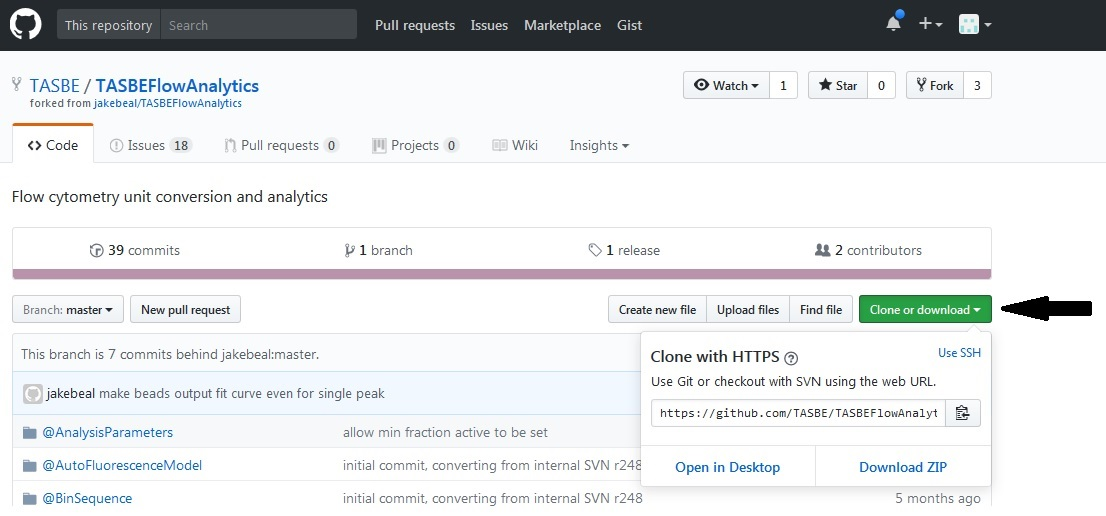
\includegraphics[width=.90\textwidth]{figures/Download_fig}
\end{center}

%The following steps can be used to install the software using \textit{Git}: 
% \begin{enumerate}
% \item If the user is \textbf{NOT} \textbf{cloning} the repository through the terminal, then please go to \textbf{Step 2}. Otherwise, locate to the directory where the repository should exist and type the command: \textbf{git clone $<url\space copied>$}. 
% \item To \textbf{clone} using the GUI client, then select \textbf{File}, then select \textbf{Clone repository}. Under the window that pops up, enter the url given and locate to the path of where the repository should exist. 
% \end{enumerate} 




\section*{SETTING UP MATLAB ENVIRONMENT}

After the \textit{TASBEFlowAnalytics} software is installed, importing the tool into MATLAB is necessary in order to use it. 

Users will direct MATLAB to where the installed software is located by first selecting \textbf{Set Path}. This step will prevent from having to re-setting the path to the installed software for every use. 

\begin{center}
  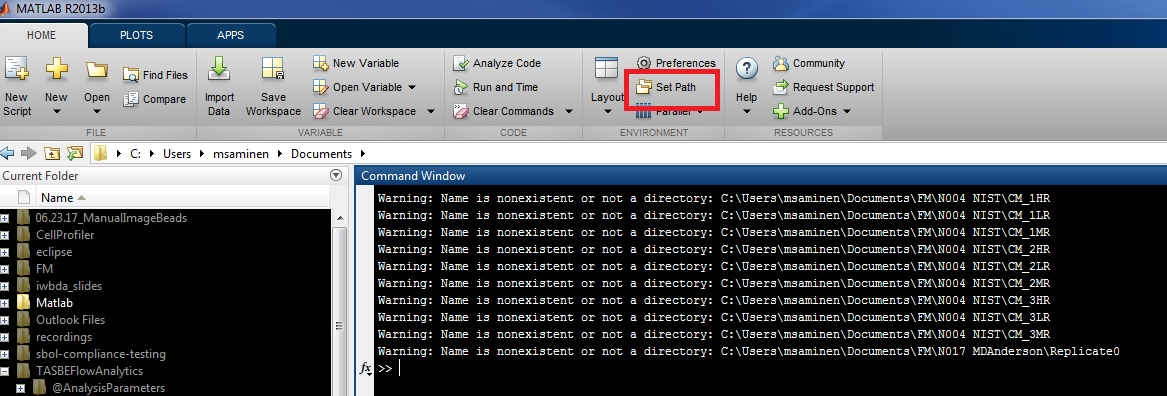
\includegraphics[width=.90\textwidth]{figures/Set_Path_Fig}
\end{center}


In the window that opens, select \textbf{Add with Subfolders} as shown below. After selecting this option, find where \textbf{TASBEFlowAnalytics} software is located and select the directory.    

\begin{center}
  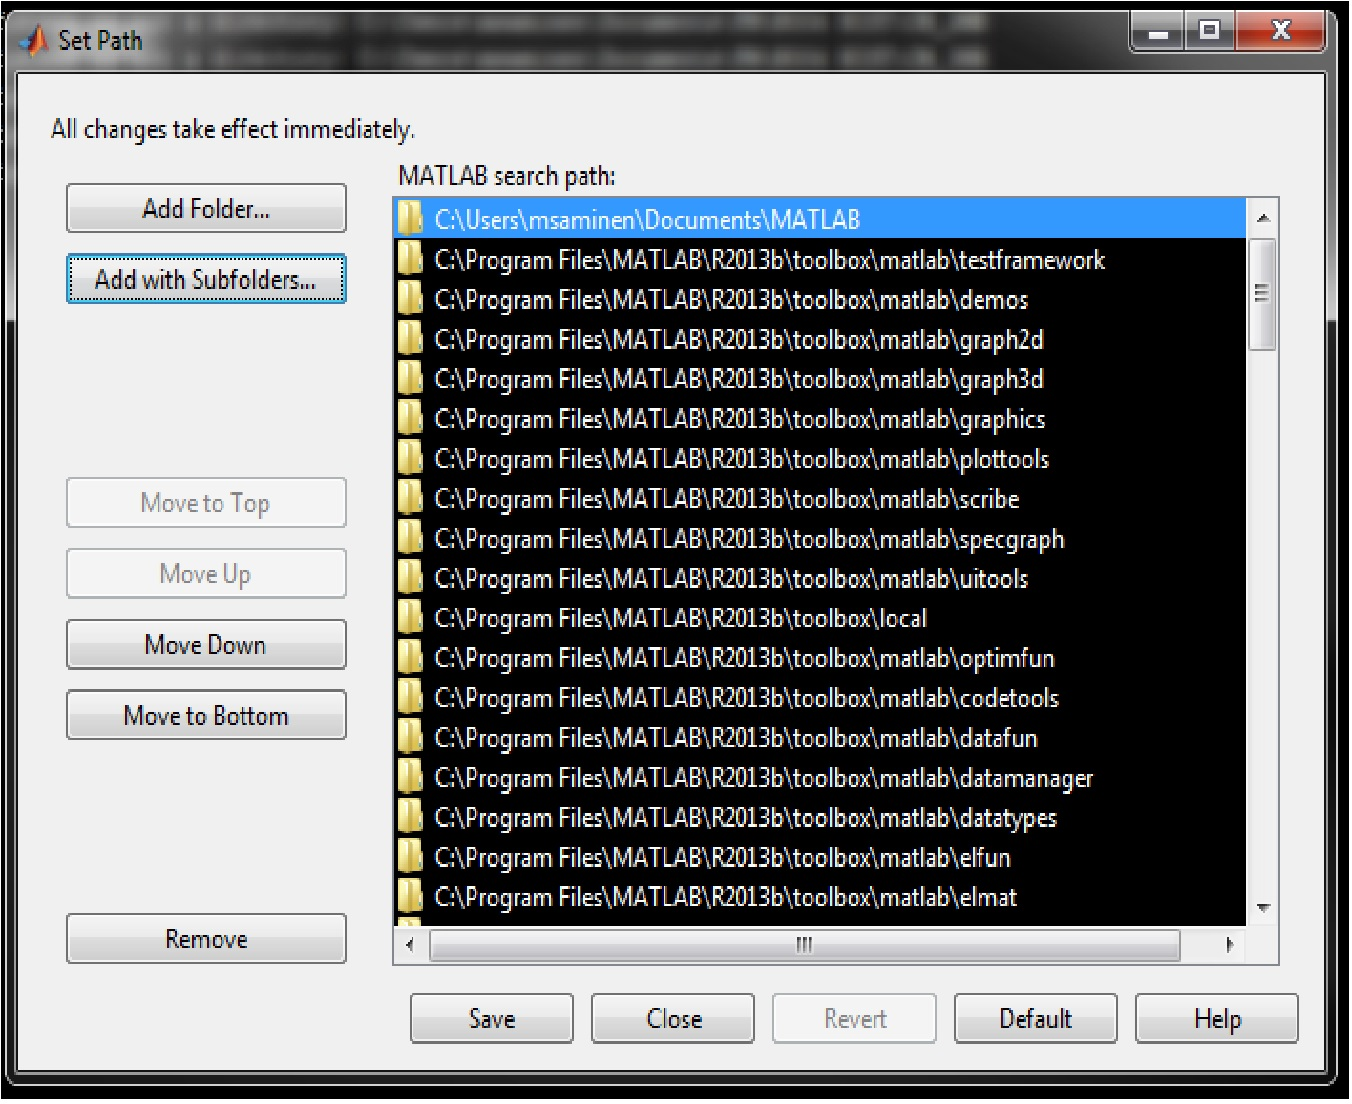
\includegraphics[width=.90\textwidth]{figures/Adding_SubFolders}
\end{center}

\begin{center}
  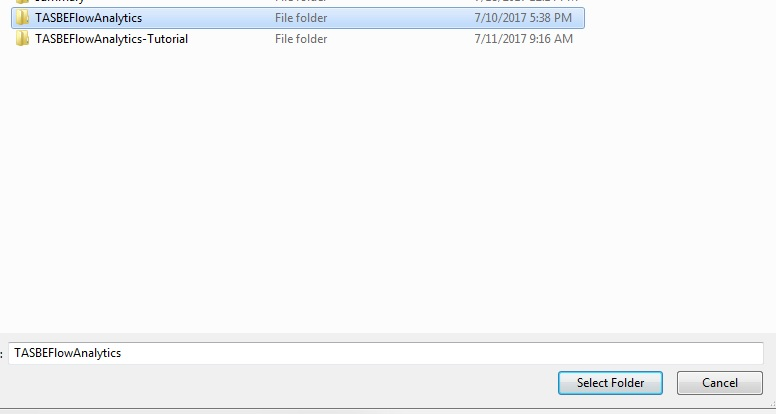
\includegraphics[width=.90\textwidth]{figures/Select_TASBE}
\end{center}

The next and final step is simply saving the changes made and closing from the window. 

\begin{center}
  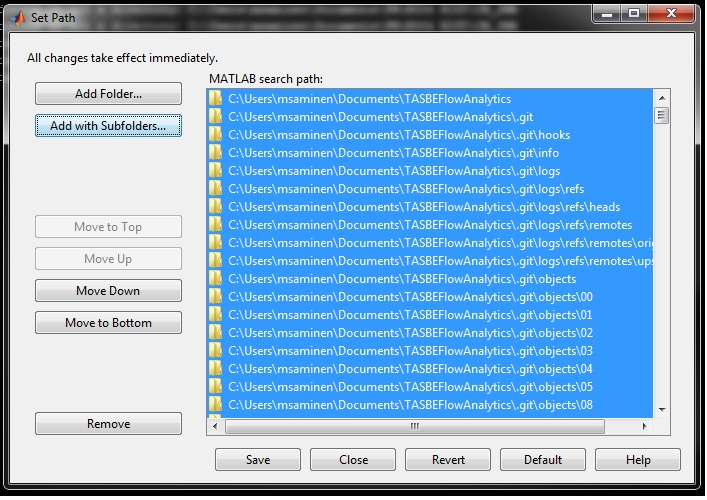
\includegraphics[width=.90\textwidth]{figures/Save_Close}
\end{center}

Users should have successfully installed and setup the \textit{TASBEFlowAnalytics} software tool within MATLAB. If there were any problems or questions, users are urged to enter issues using the \textit{Github Issue Tracker} which can be found \href{https://github.com/TASBE/TASBEFlowAnalytics/issues}{here}. Furthermore, there is an additional tutorial explaining how to use the major functions provided by the \textit{TASBEFlowAnalytics} software and troubleshooting tips for issues that users might run into. This tutorial can be found here. 
%NOTE second tutorial hasn't been created.
























